\documentclass[12pt,conference,a4paper,twocolumn]{IEEEtran}
\usepackage[left=2cm,right=2cm,top=2cm,bottom=2cm]{geometry}
\usepackage[utf8]{inputenc}
\usepackage[english]{babel}

\usepackage{amsmath}
\usepackage{amsfonts}
\usepackage{amssymb}
\usepackage{graphicx}
\usepackage{listings}
\usepackage{cite}
\usepackage{hyperref}
\hypersetup{colorlinks=false,linktoc=all,linkcolor=blue}
\usepackage{textcomp}
\usepackage{xcolor}
\usepackage{algorithmic}

\definecolor{mygrey}{gray}{0.97}
\lstset{
  basicstyle=\tiny,
  columns=fullflexible,
  breaklines=true,
  postbreak=\mbox{{$\hookrightarrow$}\space},
  backgroundcolor=\color{mygrey},
  numbers=left,
  xleftmargin=3em,
  framexleftmargin=3em,
  %frame=single,
  %language=Matlab, 
  tabsize=3,
  escapeinside={\%latex}{\%latex},
}


\title{Control and Instrumentation Laboratory (EC692)\\Assignment No.: 2}
\author{	\IEEEauthorblockN{Dhiman Sarkar}
			\IEEEauthorblockA{\\
							Roll: 19101105086\\
							Dept. of Electronics and Comm. Engineering\\
							Jalpaiguri Government Engineering College\\
							Email: ds2286@ece.jgec.ac.in
							}
			\and
			\IEEEauthorblockN{Alok Barman}
			\IEEEauthorblockA{\\
							Roll: 19101105087\\
							Dept. of Electronics and Comm. Engineering\\
							Jalpaiguri Government Engineering College\\
							Email: ab2287@ece.jgec.ac.in
							}
			\and
			\IEEEauthorblockN{Alka Tigga}
			\IEEEauthorblockA{\\
							Roll: 19101105088\\
							Dept. of Electronics and Comm. Engineering\\
							Jalpaiguri Government Engineering College\\
							Email: at2288@ece.jgec.ac.in
							}
			\and
			\IEEEauthorblockN{Azizul Mallick}
			\IEEEauthorblockA{\\
							Roll: 19101105089\\
							Dept. of Electronics and Comm. Engineering\\
							Jalpaiguri Government Engineering College\\
							Email: am2289@ece.jgec.ac.in
							}
		}

\begin{document}
\maketitle
\begin{abstract}
	Perform various tasks assigned by the instructor.
\end{abstract}

\section{Brief Description of The Assignments}
\begin{enumerate}
\item\label{p1} Consider the closed-loop system defined by $\frac{2\zeta s +1}{s^2 + 2\zeta s + 1}$ where $\zeta=$0.2, 0.4, 0.6, 0.8, and 1.0. Using MATLAB, plot a two-dimensional diagram of unit-impulse response curves without using impulse command.


\item\label{p2}  Plot the root locus of the following system $G(s)H(s) = \frac{K}{s(s+1)(s+2)}$


\end{enumerate}

\section{MATLAB Scripts}
Exercise - 1 \
Since the Laplace Transform of Unit Impulse is 1, the output of the system is same as the system function. So to get the response (i.e. in time domain), we performed a Inverse Laplace Transform and plotted the response.
\lstinputlisting[firstline=3,name=MATLAB]{ctrl2.m}
Exercise - 2
\lstinputlisting[firstline=3,name=MATLAB]{ctrl3.m}


\section{Output Results and Plots}

\begin{figure}[h]
\centering
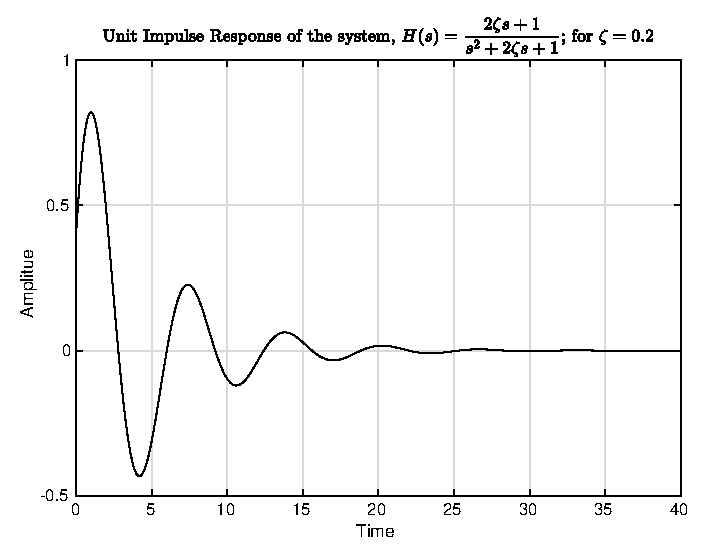
\includegraphics[width=2.5in]{z.2.eps}
\caption{Impulse Response of the system described in Problem.\ref{p1} for $\zeta=0.2$}
\end{figure}

\begin{figure}[h!]
\centering
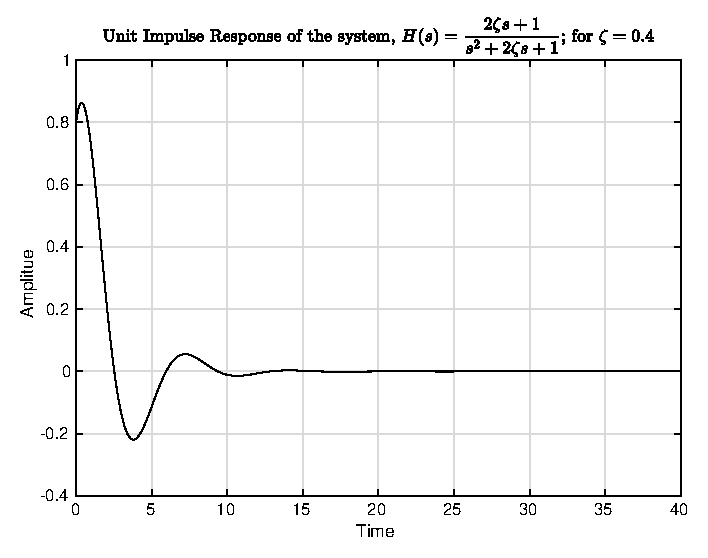
\includegraphics[width=2.5in]{z.4.eps}
\caption{Impulse Response of the system described in Problem.\ref{p1} for $\zeta=0.4$}
\end{figure}

\begin{figure}[h!]
\centering
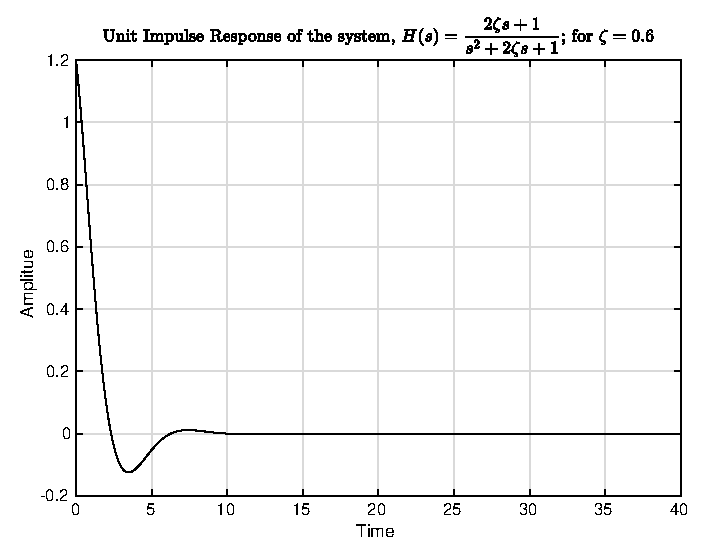
\includegraphics[width=2.5in]{z.6.eps}
\caption{Impulse Response of the system described in Problem.\ref{p1} for $\zeta=0.6$}
\end{figure}

\begin{figure}[h!]
\centering
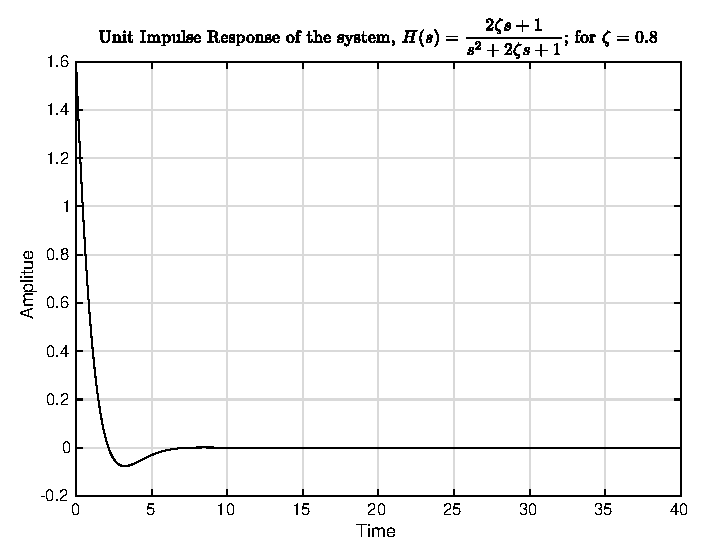
\includegraphics[width=2.5in]{z.8.eps}
\caption{Impulse Response of the system described in Problem.\ref{p1} for $\zeta=0.8$}
\end{figure}

\begin{figure}[h!]
\centering
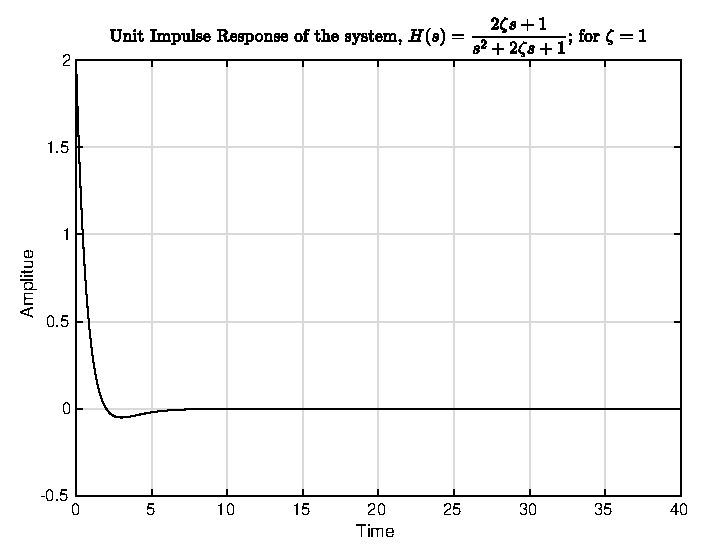
\includegraphics[width=2.5in]{z1.0.eps}
\caption{Impulse Response of the system described in Problem.\ref{p1} for $\zeta=1.0$}
\end{figure}

\begin{figure}[h!]
\centering
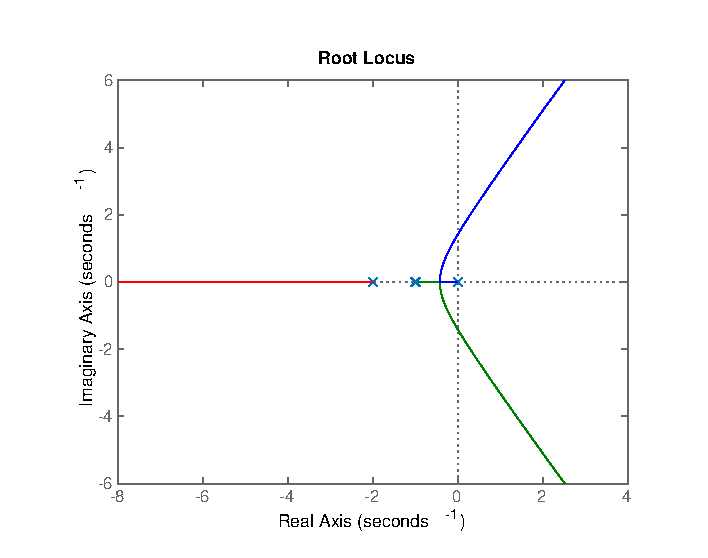
\includegraphics[width=2.5in]{rl.eps}
\caption{Root Locus of the system for described in Problem.\ref{p2}}
\end{figure}


\newpage

\section{Observations \& Conclusion}
\begin{enumerate}
\item From the first experiment we can observe that the system is oscillatory for lower values of $\zeta$. But for higher values of $\zeta$ ($\geq 1$) the system response in very snappy.
\item From the Root Locus plot of the second system described in Problem.\ref{p2} we can clearly see that the system has three poles and it has both real and conjugate complex poles.
\end{enumerate}

\section{Acknowledgment}
We would like to express our sincere gratitude to our course instructor Mr. Mirwaiz Rahaman and Mrs. Purba Basu for providing their invaluable guidance, comments and suggestions.

\end{document}